\chapter{Data entry in an office setting}\label{ch:Study1}
\begin{mynote}
\subsubsection{Chapter outline}

This chapter reports an interview study on understanding data entry work in a naturalistic office setting, and a contextual inquiry study on how people self-interrupt in this setting. Together these studies show that people try to avoid task-irrelevant interruptions, and postpone physical inquiries if they expect them to take a long time, but digital inquiries are addressed immediately. These findings suggest that people do not always know how to effectively manage self-interruptions if they are seen as part of the same activity, because of preconceptions about ease of access, and because of lack of awareness of time spent on digital interruptions.
%Together these studies show that participants have to look up information from sources with differing levels of time costs. Whereas for paper sources, time costs affect whether it is addressed now or later, they interrupt immediately to gather digital information. This suggests that people are unaware of the time spent on digital interruptions. 

\end{mynote}
Prior research has shown that the type of task influences how people manage information and therefore might impact how they address inquiries \citep{Bondarenko2005}. To address the aim of this thesis, which is to understand how the disruptiveness of inquiries for data entry can be reduced, it is therefore important to not only look at people's data entry performance using a well-structured task, but also at data entry in the environment in which these tasks are normally performed. The aim of the studies reported in this chapter was therefore to get a detailed understanding of data entry work in a finance office setting and how people currently self-interrupt. In particular, the aim of Study 1 was to get a baseline understanding of data entry work and the type of information sources they need. People were interviewed at their workplace. The aim of Study 2 was to understand the different time costs associated with information sources, and whether this affected people's self-interruption behaviour. Study 1 revealed that a major aspect of data entry work in this setting is collecting information from multiple sources with different levels of access, which then became the focus of the rest of the thesis. The contextual interview study showed office workers regularly interrupt themselves as soon as they realise they need digital information, but barely interrupt themselves to access paper sources as there is effort involved. Digital interruptions took longer than intended as participants were distracted by task-irrelevant information.

\section{Study 1: Understanding data entry work in a financial office}\label{ch:Study1}
 
\textit{This study and its results have been published in \citet{Borghouts2017} and were presented at the European conference on Computer-Supported Cooperative Work in 2017.}
 
\subsection{Introduction}
As data entry is a common task and it is important this is done both accurately and efficiently, work has been done to design and optimise data entry interfaces to support fast and accurate data entry \citep[e.g.][]{Oladimeji2013, Vertanen2015, Wiseman2013a}. Studies have shown that creating interfaces to slow down data entry \citep{Gould 2016b}, by requiring additional information \citep{Wiseman2013a} or using alternative input technology \citep{Oladimeji2011} can all reduce error rates in the lab. However, these solutions do not always work outside of the lab \citep[e.g.][]{Gould 2016b}, as it is not just the data entry interface that determines efficiency and accuracy but also other aspects of the task, such as the environment within which it is conducted \citep{Payne2013, Randall2014}. For instance, in lab studies, users are given clear instructions and are given the data to enter. In everyday computer use, data entry tasks might not be so clearly prescribed \citep{Evans2012}. To illustrate, \citet{Evans2012} investigated if people's data entry behaviour in a lab setting was comparable to how they would normally perform these inputting tasks in their everyday life. They remotely observed people's input behaviour on their personal computer, and compared this with their performance on similar tasks in a lab. Participants installed a tool on their personal computer which logged all data entry and mouse pointing behaviour they performed in one work week. Examples of tasks that were carried out were sending personal messages to friends and browsing the web. There were no differences in uncorrected errors or data entry speed between the lab and the field, but they did find that participants corrected more errors in the lab. This study shows that people check and correct their entries more when they are in a controlled environment and are focused on the task, though the measured behaviour on people's personal computers mostly included tasks where accuracy may not have been considered important, such as sending an informal chat message to a friend. 

The aim of Study 1 was to get a grounded understanding of people's data entry work in an office setting. As the nature of this first study was exploratory, interviews were considered to be an appropriate method for this purpose. Participants were able to further explain their strategies and discuss challenges they experienced. Furthermore, it enabled to collect participants' experience with past critical incidents, which may not be captured in observational sessions. The study explored people's data entry work overall, and the focus of this study was not specifically on people's information behaviour. As data collection and analysis progressed, information collection was found to be a large and integrated part of people's data entry work, which could potentially influence their performance.

The user group of this study were office workers at finance administration offices at two public universities, who conduct data entry tasks as part of their daily work.  This user group was chosen as they have a lot of data entry tasks as part of their job, and it is an area where it is important to enter data accurately, but there is also time pressure to finish work on time. Furthermore, it was an accessible user group to approach.

\subsection{Method}
\subsubsection{Participants}
Nine participants (four male) took part in the study. They were employees from two public universities and their work involved receiving various requests for payment, checking the information of these requests was correct, and entering the information along with administration data into computer systems. Ages ranged from 18 to 52 (two participants wished to not disclose their age). Their level of experience differed, with some participants having just started doing this type of job and other participants working in Finance for 17 years. All but one worked full-time. Table \ref{table:ch3_participants} shows further demographic details of the participants. Typical data entry tasks participants dealt with were checking and entering expense forms sent by staff and students, paying salaries and pensions, controlling research budgets, monitoring university income and expenses and entering employee information. Participants were recruited by sending invitations to opt-in mailing lists of Finance departments, and were reimbursed with a \pounds10 Amazon voucher.

\begin{table}
\caption{Participant information.}
\centering
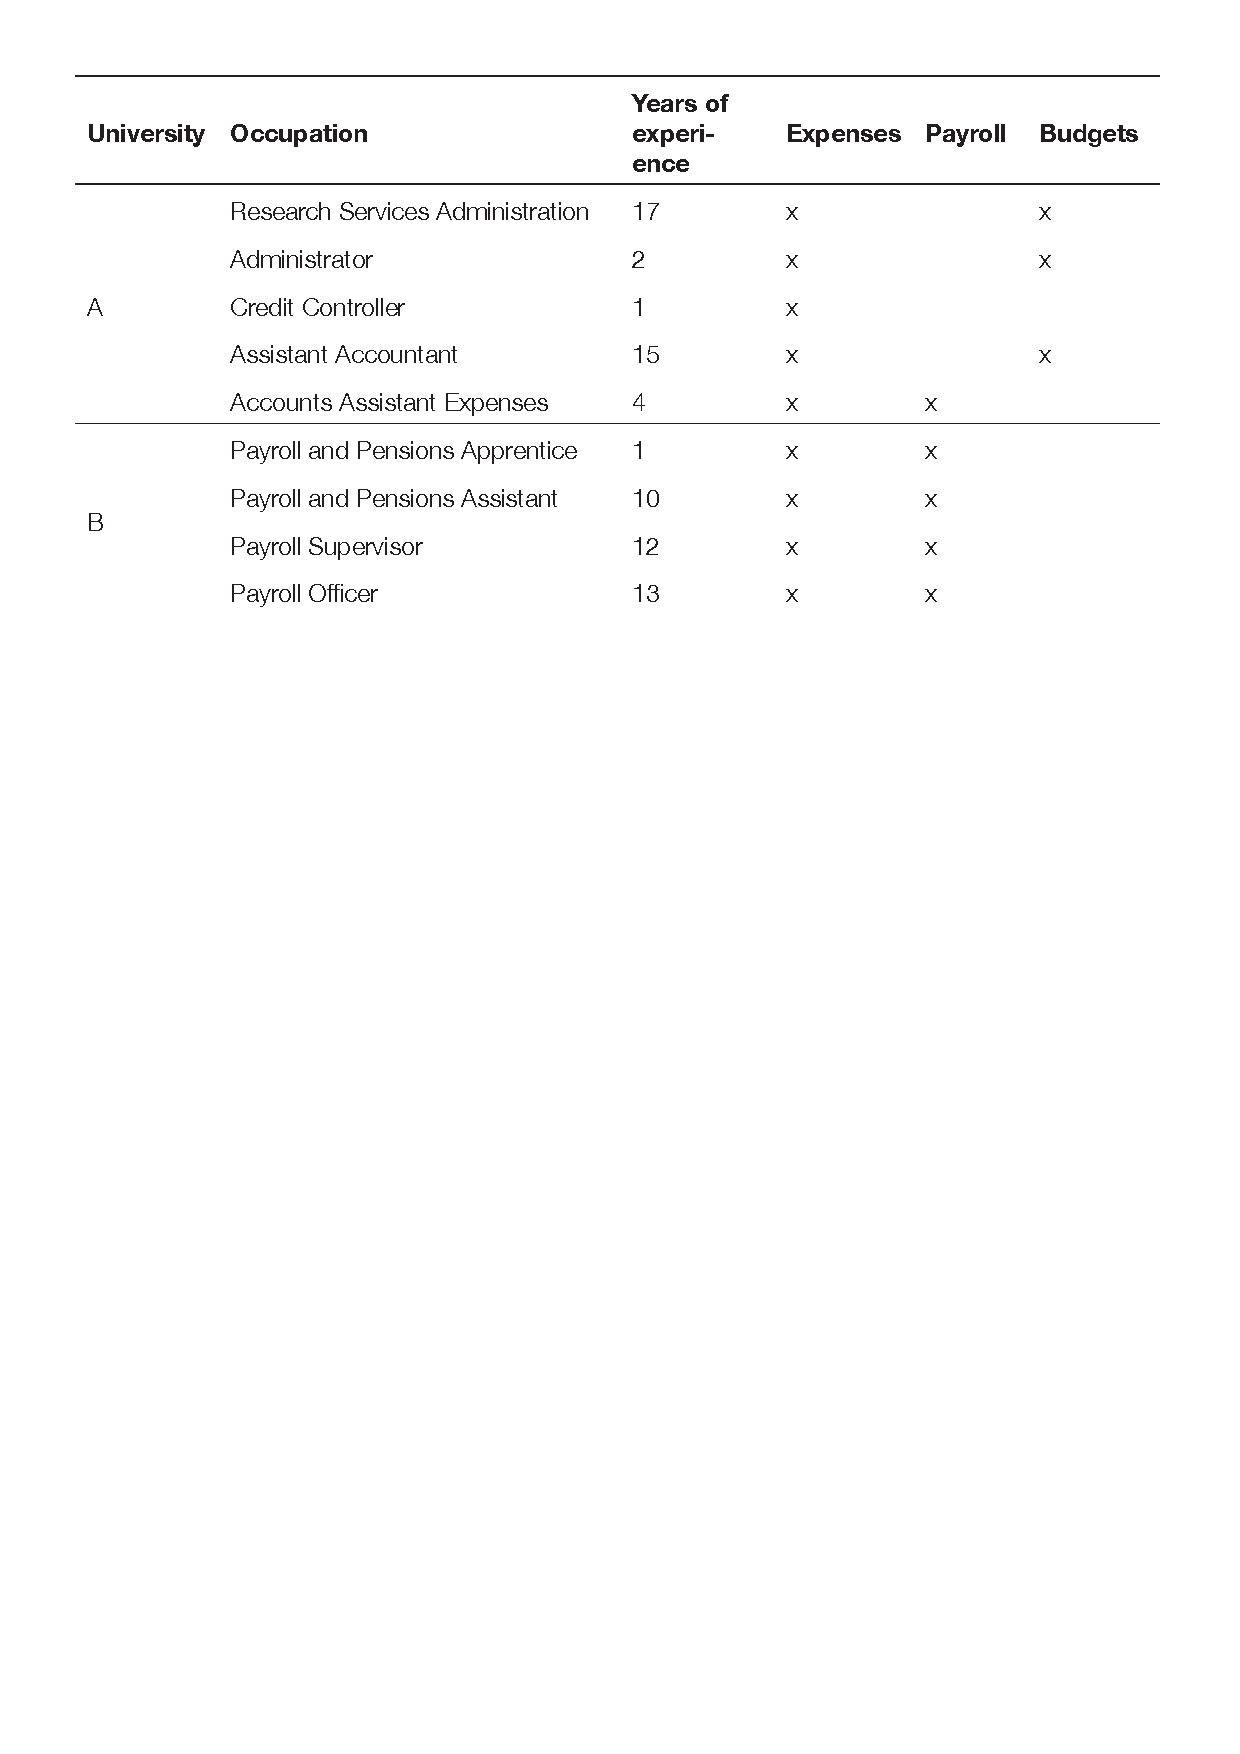
\includegraphics[width=0.9\textwidth]{images/ch12/Study1-Table1.pdf}
\vspace{-3pt}
\label{tbl:ch12-Table1}
\end{table}

\subsubsection{Materials}
Materials that were used during the interview were a voice recorder, a paper copy of an interview script with the interview topics and guiding questions, a consent form, an information sheet for the participant and a notebook and pen to make notes. The interview script, information sheet and consent form are included in Appendix \ref{ch:information_sheet}.
Each interview covered four guiding topics, which are briefly described in Table \ref{table:ch3_interviewtopics}. For each topic, a number of questions were written out beforehand. These questions were used as a starting point to get the participant talking and guide the interview. Based on what the participant was saying follow-up questions were asked. The audio transcription program ExpressScribe was used to transcribe the interviews. The data analysis programs Nvivo and Atlas.ti were used to analyse the data. Nvivo was used to code the interview transcripts and notes. Atlas.ti was used to complement the analysis in Nvivo and allowed to identify relations between codes.

\begin{table}[htp]
\centering
    \begin{tabular}{ | l | p{10cm} |}
    \hline
     Topic & Description \\ \hline
    Job description & A description of the tasks that the interviewee deals with. The purpose of this topic was to start the interview easy and give the interviewee the opportunity to explain what their job entails. \\ \hline
    Number transcription & This includes questions on when and how people typically enter numbers for work.  \\ \hline
Environment & This topic includes people's physical work environment, and the organisation they are a part of. \\ \hline
Demonstration &  Interviewees were asked to give a demonstration of entering data into their system. The aim of this part of the interview is to see the type of data entry tasks people have to do, and also gives a chance to see the information sources and systems people currently use. \\
    \hline
    \end{tabular}
    \caption[Study 1 interview topics]{Interview topics.}
    \label{table:ch3_interviewtopics}
\end{table}%

\subsubsection{Data recording}
A voice recorder was used to audio record the interviews. One participant wished to not be audio recorded and one interview could not be audio recorded due to technical issues, so for these two interviews notes were taken of the answers. For the remaining seven interviews, notes were only made of observations and not the participants' answers. Notes were made with pen and paper. Photographs were made of the work environment and screenshots of the systems that the interviewees used.

\subsubsection{Interviewing procedure}
The interviews took place at the participants' workplace. For two interviews, the interviewee's office place was not suitable for talking so the interview took place in a common room nearby, and these participants showed their workplace and completed a demonstration of entering data after the interview. Participants were welcomed and informed about the study. They received a paper information sheet with the outline of the study and contact details of the researcher to keep for future reference. They were also asked to read and sign a consent form.

The interviews were semi-structured and took between 20 and 55 minutes. Each interview was reviewed afterwards, and findings sometimes fed into new questions being included or some questions being adapted in subsequent interviews.

\subsubsection{Pilot interview}
A pilot interview was conducted with an acquaintance of the researcher who worked in Finance, to test out the set-up of the study and questions. The interview took place at the participant's home, notes were taken with pen and paper, and the interview was audio-recorded using iMovie on a Macbook Pro. 

Taking notes slowed down the flow of the interview: sometimes the interviewee stopped talking to give the interviewer the opportunity to finish taking notes. Furthermore, taking notes took attention away from what the interviewee was explaining: assumptions made during the interview did not seem to be accurate in later analysis. Therefore, it was decided that note taking would be kept to a minimum. Notes would only be made of observations that could not be taken from audio recordings.

%The interviewee talked elaborately about manually converting different currencies, and identified this task as the main place where errors occurred. Therefore, questions were included about if interviewees dealt with foreign currencies and converting these. 

\subsubsection{Ethical considerations}
The study was undertaken with ethical approval from the UCL Research Ethics Committee [Project ID Number UCLIC/1415/001/Staff Brumby/Borghouts]. 
At the start of each interview, participants were first informed verbally about the study. They were then given a consent form to read and sign, and were given an information sheet to keep. This information sheet contained the study information and contact details of the researcher and the project's principal researcher, should participants have any further questions after completion of the study.  They were asked permission for the interview to be audio recorded. One participant wished not to be audio recorded and notes were taken instead. 

Participants were informed that the data would be used for research purposes only and stored in accordance with the Data Protection Act 1998. They were also informed that their data would be anonymised and when used in a report or academic paper, their data would not be directly identifiable. Names of participants or the universities they were working at were not included in the interview notes and transcripts.
 
\subsection{Results}
\subsubsection{Data analysis}
After each interview or set of interviews, a first analysis took place. The audio recording was played back, notes were typed into a digital file and reviewed and the interview was transcribed verbatim. Several non-verbal cues were included in the transcription as well, such as when the interviewee laughed or sighed, as well as descriptions of when the interviewee was demonstrating something. The advantage of doing the transcription shortly after the interview was that it was still easy to remember from listening to the audio recording what was being demonstrated. Interesting findings and initial patterns that were apparent across the data were written down. 

After all interviews had been transcribed, the transcriptions and notes were printed and the data was analysed using thematic analysis \citep{Braun2006}. An inductive approach of thematic analysis was used: there was no pre-existing coding scheme, and codes were created based on what emerged from reading over the transcripts and notes. Anything in the data that was considered to be interesting was annotated by hand and labelled with an appropriate code. On reviewing the coding, some codes were grouped together in one code, additional codes were named, and similar codes were grouped under themes. For instance, an initial code was Notifications, such as e-mail notifications. During the second coding iteration, it was identified that people always talked about notifications in the context that they were interrupted (by a notification) rather than about notifications on its own. Therefore, notifications and interruptions were grouped into one code. 

The themes were then reviewed, to see if they addressed the purpose of the study. The transcripts and notes were then imported into Nvivo and coded digitally. Atlas.ti was used to complement this analysis and allowed to identify relations between codes. 

\subsubsection{Themes}
In total 51 codes were derived, and these were grouped into 8 main themes, which are listed and described in Table \ref{table:ch3_themes}. If codes or separate quotes did not belong in a certain theme but were still considered relevant, they were grouped in the Other category. 

\begin{table}[htp]
\centering
\resizebox{\textwidth}{!}{
    \begin{tabular}{ | p{3cm} | p{8cm} | l | l |}
    \hline
     \textbf{Theme} & \textbf{Description} & \textbf{Quotations} & \textbf{Participants} \\ \hline
     Task characteristics & People described things that were particular to their task, for instance how they structured their task, whether they switched tasks, and how long they took to complete tasks.  & 129 & 9 \\ \hline
	 Checking & People talked about checking data input as part of their job. & 103 & 9 \\ \hline 
	System & People talked about the computer system they were using to input data.  & 91 & 9 \\ \hline 
		Environment &People described their environment, for instance they talked about their physical work setting, and the work culture of their organisation. & 80 & 9 \\ \hline 
		Data &People described the data they were dealing with, for instance the type and length of data items, and from which source they copied data. & 75 & 9 \\ \hline 
		Errors &People described situations where errors were made: who made them, why were they made, what were the consequences. & 75 & 9 \\ \hline 
					 Strategy & People described the strategies they used to carry out their task.  & 54 & 9 \\ \hline 
		Importance of accuracy and paper trails &People talked about the sensitivity of financial data which is why not all people are authorised to approve or access financial data, and the importance of a paper trail for data entries. & 35 & 8 \\ \hline 
			 			 Other & People talked about things that did not fit into any other category but were still considered relevant, such as issues they experienced, or queries they often received.   & 74 & 9 \\ 
    \hline
    \end{tabular}
    }
    \caption[Study 1 Themes]{The themes, along with a description. The column Quotations indicates how many times this theme was brought up during interviews, and the column Participants indicates how many participants talked about it.}
    \label{table:ch3_themes}
\end{table}

Each theme was visualised as a diagram, which is included in Appendix \ref{ch:S1_Diagrams}. Each diagram shows a theme's main codes and relationships between codes, the number of quotes that were grouped under this theme, and the number of interviewees who mentioned it. These diagrams helped to gain insight how codes were connected, and also how prevalent topics were across the collected data. In the following Results section, I report the key findings from the analysis.  The diagrams are included in the Appendix to make transparent how data was analysed and to clarify what I base the key findings and conclusions on. 

I first describe the data entry work participants dealt with, to provide context to the type of work I focus on in this thesis. I then discuss how people scheduled their work, the information sources they dealt with, and current strategies to improve data entry performance.

\subsubsection{Type of data entry tasks}
A common data entry task was processing expenses. Interviewees received requests from university staff and students, who had spent money for research purposes and wanted to claim back the expenses. Participants had to check the information they were given was correct. For instance, they had to check that the amount being claimed back matched the value on the original receipts, and that the expense fell within permitted limits. In addition to transcribing and checking individual numbers, participants also mentioned they often have to perform and check calculations, for example to check that all individual expenses were converted correctly from a foreign currency. After checking the data and calculations, they then had to enter the data, along with other information such as budgeting and staff information, into a computer system. The time spent on processing one expense claim differed: checking data on a short expenses form could be completed in two minutes, while a single manual calculation could take between 20 and 30 minutes. Two participants described dealing with a lot of data entry as time-consuming and tiresome.

People primarily dealt with numeric data, such as financial data and IDs. The monetary numbers they dealt with ranged from five to millions of pounds. Participants also entered and checked alphanumeric and non-numeric data such as employee names, addresses and bank account details. Numeric data consisted of individual numbers, as well as groups of numbers that together made up a new number, such as the total amount of money spent on a project. Participants had to both check and transcribe each individual number, and check that the calculation was correct. 

\subsubsection{Scheduling data entry work}
The workload varied throughout the year. Four participants mentioned that their work followed a work cycle, which meant they did different things at different times of the month. One week could be reserved for checking all the data they received from another department, while another week could be spent on solely inputting data. On average participants reported that they dealt with between 30 and 80 expense claims per day. The amount of individual data items to enter averaged to 6,000 items a day. 

To complete data entry work efficiently, eight participants saved up data entry tasks, to enter all data in one sequence. If they received new data entry tasks, they often did not work on them immediately, but instead waited until they had several saved up and then completed all of them in a single batch. P2 was the only interviewee that processed forms with numbers to enter as they came in. She only dealt with a couple of claims per day, and did admit that if she had more data to fill in, she would probably do it in a more efficient way.

The reason for batching data entry work was that participants found it quicker and easier to do the same type of task in one sequence, before they started another type of task. Participants did not have specific deadlines set by their organisation to finish certain expenses. Some said they saved them up but did try to finish expenses before the next payroll was due, so that claimants could get their expenses reimbursed on time. P6 explained he postponed processing expense forms until the deadline to submit forms for that month has passed, after which he did all forms in one sequence: \textit{"When I’m doing it lots at a time, I think once you get into sort of the hang of it, it gets done a lot quicker."} (P6)

\subsubsection{Interruptions}
Participants batched data entry work, and while doing this work, tried to concentrate on the task at hand: they avoided self-interruptions to other tasks: \textit{"I try to concentrate on my task...I try to do one task (i.e. doing all expenses), finish one, and then do another."} (P9). All participants did attend to some external interruptions, which they considered part of their job: P8 had to pause his task immediately if a staff member entered his office and needed his help. Other participants mentioned they primarily tried to concentrate on the task at hand, but did briefly glance over e-mail notifications, to see whether something important needed their attention.

\subsubsection{Information sources}
While participants avoided task-irrelevant interruptions during a data entry task, they did have to interrupt and leave the data entry system to look up information related to the task and then get back to the system window to enter it. The information needed for one task was usually spread over several windows on the computer, so participants had to flick back and forth or memorise certain information from one window to use in another window: \textit{"Depending on the input, it can be quite complicated, and there are quite a lot of different screens to input."} (P7). All participants had their computer windows maximised, so one window covered the whole screen and participants could not look at the data entry window and information source concurrently. Participants said that if they had to get out of the system to look up information digitally and then get back to the system window to enter it, they preferred to memorise the information, rather than flick back and forth and look it up each time they needed it: \textit{"I wouldn't necessarily have to [memorise it], it's more (…) if you have to keep flicking back to different things, it's sometimes just easier to try and remember it. But you can obviously take the long version and keep flicking back to the correct screen."} (P3). Data items that had to be entered frequently such as project codes, were memorised even if participants did not deliberately choose to do so.

The data was spread across both digital as well as paper sources, and participants had to switch between computer windows and physical locations to retrieve all data required for a single expense claim. Examples of digital sources were spreadsheets, Word documents, departmental databases and e-mails. Examples of paper sources were receipts, claim forms, and print-outs of spreadsheets. Participants worked with paper sources for two main reasons. First, digital information was printed out to keep it nearby. P7 and P8 had printed out information they frequently needed to look up and had placed this nearby on their desk, so they could easily use this to check if the input they had received was correct. Second, some documents had to be in paper form for auditing purposes, because participants were working with sensitive financial data. Hard copies of receipts and signed paper claim forms had to be archived and were checked by external auditors. People also explained they liked to write out and keep a record of manual calculations, in case someone had any questions on how figures was calculated.

\subsubsection{Checking for data entry errors}
Even though participants discussed they tried to focus on data entry tasks by avoiding task switches, they did discuss that data entry errors still happened frequently. Errors that were made were typos, miscalculations, or the wrong information altogether. The main explanation people gave for errors was that it is human to make mistakes, but it was also mentioned people are under time pressure, and that people rely on the fact it will be checked by another person, which makes them less careful in entering accurate data. P9 attributed it to having to switch between computer windows: \textit{"If you, by mistake, just left that menu, went into another linking menu that comes up with somebody else's payroll number, you would never know that you're inputting somebody else's calculation into another record. You have to be so careful."} P4 attributed errors to the use of both paper and digital files: he felt it was much easier to make an error and omit figures when transcribing from paper sources.

Errors had negative consequences on people’s work. If an error was spotted and was sufficiently small, it could be processed or corrected without negotiation, but if it was a large error, it had to be sent back or forwarded to a higher authority for approval. This considerably slowed the process down. Furthermore, P8 warned that even with extra human checks not all errors get caught, which meant errors could be made with paying back claimants.

The main method to prevent errors was to have data input visually checked by multiple people before it was processed for payment. People's experience with this checking system differed: P3, a credit controller who was one of the first people on her team to enter the data before it went to another colleague, believed it increased the chances of an error being caught because it goes through so many different checks. In contrast, P8 and P9 argued this made people even less careful about making errors. As payroll supervisors, they were the last persons at their office to check data before it was submitted to the system and processed for payment. They commented that even at this last stage it was still quite common to spot data entry errors: \textit{"The departments actually sometimes treat us as a checking system [laughs], but they shouldn't really. (…) even though we are like a second check, we feel sometimes that we are the first checkpoint."} (P9).

\subsection{Discussion}
The purpose of this study was to gain a better understanding of data entry work in financial offices, and the physical environment in which these are conducted. For this purpose nine interviews were conducted with office workers from two public universities who worked with financial data. The main findings of the study are: 

\begin{itemize}

\item 
people batch their work to enter a lot of data entry at once, and minimise interruptions to other tasks. 
\item 
people have to interrupt to get the data to enter from multiple information sources
\item 
data entry errors are common, and the current solution is to have data entered and checked by multiple people before it gets submitted to the system
\end{itemize}

I first compare the findings with prior research, before concluding what we learn from this study. 

\subsubsection{Batching data entry work}
Though participants received data entry tasks on an ad-hoc basis, most of them saved them until a specific moment and then processed them all in a bulk. People stated that it made them faster in entering data, and they preferred to focus on one task at once. Prior experiments have shown that people do become faster in data entry over time, but also more erroneous \citep{Healy2004}. Data entry interfaces that slow people down have been shown to reduce errors (e.g. Gould et al., 2016; Oladimeji et al., 2011), but these lab studies tested up to 240 number entries, whereas participants in the current study reported they often had to enter around 6,000 numbers a day. Interfaces that slow people down may therefore not be applicable in the setting of the current study. \citet{Healy2004} recommend regular breaks when entering large amounts of data to maintain accuracy. However as participants in this study were free to schedule their data entry work and deliberately chose to schedule all their data entry in one session, it may be challenging to initiate and take work breaks themselves. 

\subsubsection{Fragmentation of work}
Contrary to prior data entry research, information was not located on one source but was scattered across physical and digital information sources. Furthermore, in data entry experiments people are often only presented with the data they have to enter and sometimes are given only one data item at a time. The sources from which people had to enter data in this study usually contained a lot of data, not all of which was relevant to the task: sometimes participants had to go through a large spreadsheet, before they found the number they needed to copy. The amount of irrelevant data on the sources can increase the time people need to look up the information they need. 

This fragmentation of work is consistent with prior workplace studies that found  office work often involves switching between different sources \citep{Cangiano2009, Czerwinski2004, Mark2005, Sellberg2014}. In the current study, the time cost to access these information sources also differed. For instance, some paper sheets were on people's desk, but some paper sheets had to be retrieved elsewhere. Participants also dealt with multiple windows on their computer screen, and sometimes needed to switch between different windows. Instead of flicking back and forth to view information they had to enter in another window, participants said they preferred to memorise it, even though they could also write the information down or in some cases copy and paste it, which would be a more accurate strategy. This behaviour can be explained by the soft constraints hypothesis, which states that people increasingly rely on information in memory, as more effort is involved in accessing external resources \citep{Gray2006}. This strategy allows people to be faster, but carries the risk that they misremember it. In previous studies, trying to hold more items in memory during a copying task increased errors \citep[e.g.][]{Borghouts2015, Morgan2009}. However, in these studies participants had to copy unfamiliar data. In the current setting, the information had some meaning to users and some items were entered more often than others. These familiar numbers are more strongly represented in memory \citep{Wiseman2014}, in which case a memory-based strategy may be a

The understanding that entering data is only one part of the broader data entry task flow can inform future data entry research and improve the way data entry tasks are modelled in lab-based experiments. Future lab-based studies could require participants to first collect data from multiple sources, in order to see how it affects data entry performance. Having an experimental task that is more closely modelled to a situated task will give a better understanding to what extent different interventions are applicable. For example, slowing people down in data entry has shown to reduce errors in the lab \citep{Gould2016, Wiseman2013b}, but this intervention may not desirable if people are holding items in memory, or entering large volumes of data.

\subsubsection{Error checking}
Fragmented attention has been shown to have a negative effect on work performance \citep{Bailey2001, Carrier2015}, and participants reported errors happened regularly. To detect these errors, data input was visually checked by multiple people. This checking method resembles \citeauthor{Reason1990}'s \citeyearpar{Reason1990}  Swiss Cheese model, where multiple checking layers are used to minimise the risk of errors. However, prior research has shown this is a poor checking method to check for errors in data entry \citep{Olsen2008, Wiseman2013a}. Despite being widely applied in practice, there is no strong support for the effectiveness of double-checking \citep{Li2016}. One of the reasons people may not detect errors when checking a colleague's entries is confirmation bias, which occurs when people selectively attend to stimuli that confirm one's belief \citep{Lewis1986}. People may expect data entries to be correct: participants reported they regularly received erroneous data, which had previously been checked and approved by several people. 

%\subsubsection{Limitations}
%An inductive approach was taken to analyse the data. However, it should be acknowledged that no researcher approaches research data completely neutral \citep{Blandford2013b}: data analysis was informed by pre-existing knowledge of data entry literature, which partially shaped the direction of the data analysis. Furthermore, interviews were semi-structured and follow-up questions were asked based on answers of the participant. 

\subsubsection{Summary}
The aim of this study was to get a baseline understanding of people's data entry work in an office setting. Through interviews with data entry workers, I found that a substantial part of this type of work is not just entering the data but also collecting it from multiple sources. This has often been overlooked in previous data entry work, and may have an impact on data entry performance. We also learn that data entry workers treat irrelevant and relevant self-interruptions differently: interview findings suggest that they try to work efficiently and avoid task-irrelevant interruptions during data entry work. People try to batch similar data entry tasks to avoid task switches, but then have to interrupt for the task to collect information sources, which are spread across the task environment with different time costs to access them. 

The study relied on people's own explanations of their practices. This gave insight into reasons why people may employ certain strategies, and through this method I was able to discuss critical incidents which would be unlikely to be uncovered through observation alone. A limitation of relying on people's self-reporting however is that they may not do what they say they do \citep[e.g.][]{Randall2014}. Though people gave short demonstrations to support their explanations, they were not shadowed doing their work for longer periods of time. Importantly, while we know that information is scattered across the environment, it remains unclear from these interviews alone how people go about accessing these - in other words, how do they manage inquiries with different time costs? The aim of Study 2 was therefore to observe and understand how participants currently address inquiries for data entry work.

%Sometimes the cost to access an information source was low, and people could easily access it and look at it while entering it. Other times the cost was high, and people had to go back and forth between the window that showed the information, and the window in which they had to enter the information. Theory suggests that these different access costs have an impact on strategy, speed and accuracy. In previous experimental studies, an increase in IAC made people check the information source less and instead enter what was in their head. This can make people more efficient as it minimises switching between the information source and the input interface, but if the information in the head is wrong, it increases errors. In these previous studies, it increased errors, but the studies made use of abstract artificial information, which may have been too hard for participants to memorise. 
%In the current study, people had to copy numbers and text. Previous studies showed that when looking at text and/or numbers, a deeper encoding of the information in memory makes people more accurate in entering the information. 
%The next study aims to see if the effect of IAC on a copying task extends to copying numbers, which people have experience with copying and can more easily memorise.

\section{Study 2: Managing inquiries for data entry}

\textit{This study and a subset of its results are included in \citet{Borghouts2018} which is currently under review as a journal paper.}

\subsection{Introduction}
A large part of data entry work studied in Study 1 was not only entering the data, but retrieving it from the environment. People had to leave the data entry system to look up information from several sources, and hold data in memory whilst switching between documents, applications and the data entry system. 
The purpose of this study is to investigate people's current work practices to look up information from the environment for data entry work. What information do they need, and what information sources do they use? And how do they address these needs? Do they look up information as they need it, or get all the required information first and then enter it? It is important to understand how people manage subtasks of looking up information as part of data entry work, as different strategies impact task performance. 
%They may also change their strategies as they get more experienced with the task and know where to get the information from, or enter all information that is easy to access first.

The following questions will be addressed in this study:

\begin{enumerate}
\item 
What is the information needed for an expenses task?
\item 
Where is this information retrieved from?
\item 
What are the strategies people use to look up information?
\end{enumerate}

A contextual inquiry was conducted with nine finance employees from the same population as in Study 1. In this study, the specific focus was on people's information behaviour. Participants were observed at their workplace, and asked to first carry out a data entry task while thinking out loud. Next, they were observed while they continued working as they would normally.

Participants in the current study were video recorded while doing the expenses task. The video recordings captured the participants' interactions with the artefacts involved in the task, but the financial data on the information sources could not be identified from these recordings. The video recordings were used to supplement written observation notes, and after the observation part of the study, some video segments were played back to participants to explain what they were doing at certain moments.

Data was gathered and analysed using Distribution Cognition (DC) as a theoretical framework \citep{Hutchins1995}. Distributed Cognition is a theoretical framework that views cognition as distributed between people, internal and external sources and over time. 
As it takes the distributed nature of cognition as focus of analysis, it was considered it to be a useful framework for this study to help make sense of the fragmentation of, and access to, information for data entry work. 

%Despite the usefulness of DC in understanding and designing for human-computer interactions \citep{Hollan2000}, to my knowledge it has not yet been applied to data entry work. %In most data entry studies, information is given and well-defined. The focus then becomes on decreasing the access costs []. However …

To analyse the data, I followed the guidelines of \citet{Furniss2006} on constructing descriptive models of the task environment. Though the models were originally developed to apply Distributed Cognition for teamwork, the models can also be useful with an individual as the focus of analysis. In particular the Physical and Artefact model were useful in understanding the distribution of, and access to, information for the user. The methodology facilitated to identify potential issues, and better understand people’s current strategies and workarounds. 
%This study focused on understanding how information is laid out in the environment for data entry work at financial offices, and people'��s current practices to collect information, with the aim of informing design of user-friendlier systems.

\subsection{Method}
\subsubsection{Participants}
Nine participants (five male) from four different finance offices took part in the study. 

Participants from Study 1 were invited to participate again, but only one participant was able to participate again in the current study (P8 in Study 1, P1 in Study 2). 
For the remainder of recruitment, a parallel sampling approach was taken \citep{Onwuegbuzie2008}. This means participants were drawn from the same population using the same recruitment techniques, but were not the same individuals. As in Study 1, they were employees from financial offices at public universities dealing with processing expense claims. Participants had one of the following roles: research manager, payroll officer, and administrator.

People were recruited through a combination of convenience and snowball sampling. People were invited to participate via emails sent to opt-in mailing lists of Finance departments, and emails forwarded by contact persons and people who had already participated. A session with a single participant took between 2 and 2.5 hours, and participants were reimbursed with \pounds15.

\subsubsection{Site setting}
The study took place in the same type of office setting as in Study 1. Participants were recruited from the same two public universities, and one office from Study 1 was visited again in this study. The other participants were from three different offices within these universities. They worked in open plan offices with two or more colleagues working nearby. 

\subsubsection{Contextual inquiry}
My data collection was informed by using the methodological approach of contextual inquiry.
Contextual inquiry is a combination of observation and interviewing users and their everyday work, with the aim to use the findings to inform design of the systems they use \citep{Holtzblatt2014}.
\citet{Holtzblatt2014} argue that observing participants carrying out their work can reveal concrete details, and it can help participants to recall past situations of carrying out work. It is therefore considered to be an appropriate method for the aims of this thesis, as it involves understanding users' expenses work with the aim to translate it into design implications for their expenses system. 

All interviews were audio recorded, and observations were audio and video recorded. The contextual inquiry consisted of four parts \citet{Holtzblatt2014}:
\begin{enumerate}
\item 
Interview

In this part, the participant was asked general questions about their work. This part was primarily to make the participant feel comfortable and start the session easy. As I had already gained an insight on finance employees' general work in Study 1, this interview was shorter and more particularly focused on their expenses task and information sources they used. 
\item 
Transition

In this part, the participant demonstrated the expenses task while thinking out loud. I prompted the participant to elaborate what was happening if the participant fell quiet, or if something interesting or unusual happened.
\item 
Observation

During this part, the participant continued doing his/her work without being interrupted or explaining what he/she was doing and why. I observed and made notes.
\item 
Summary

In the final stage, I summarised to the participant what I had found to check if these assumptions were correct. If some parts of the observation need clarification, segments of the video recording were played back to the participant, and he/she was asked to explain what was happening at certain moments.
The participant was thanked and debriefed.
\end{enumerate}

\subsubsection{Pilot study}
In order to test the suitability of the study set-up, a pilot study was conducted with a financial administrator at a university who dealt with processing expenses. The study took place at the university, and notes were taken with pen and paper. 

Initially, the intended method of this study was to conduct a contextual inquiry, followed by a week-long diary study where office workers would log diary entries of their expenses tasks. The aim of this diary study would be to get a further insight in additional information sources they may sometimes use, that were not covered in the contextual inquiry.  Participants would submit a diary entry either by writing down a description or by taking a photograph of the task setting, showing the information sources. At the end of the day, they would have to answer the following questions about their short entries: what information did you need, where did you need to get it from, and when did you look up the information. This method built on a study by \citet{Sohn2008}, where participants kept a diary of their mobile information needs and how they addressed those needs. 

The administrator explained that expense tasks usually are conducted in the same manner, and predicted I was unlikely to find a lot of instances that differ from my observations of having office workers do the task.
Furthermore, by observing them I am able to see the access people have to the resources and how much time it takes them to get the data, as well as when in the task they decide to look up information. This information would be more difficult to get insight to through diary entries.

It was therefore decided after this study to not conduct a diary study but instead only observe office workers, and ask them to explain their work.

\subsubsection{Ethical considerations}
The study has ethical approval from the UCL Research Ethics Committee [Project ID Number UCLIC/1415/001/Staff Brumby/Borghouts]. 

Participants were invited by email. The email included details such as the purpose, duration and reimbursement, and what participation would involve. 

Before the start of each session, participants were again verbally briefed about the purpose of the study, and what would be expected of them. They were then asked to read and sign a consent form, and were given an information sheet with the study information and my contact details for them to keep. 

All participants gave permission for the session to be audio and video recorded. After the video camera was set up, participants were shown what was captured by the camera, to confirm the camera was set up appropriately. This ensured the participant that no financial data was legible from the recordings.

It was explained that the purpose of the study was to get a better understanding of how they normally go about their work with an aim to improve the system, and that there were no right or wrong ways of doing tasks. They were free to withdraw from the study at any time.
Participants were informed that the data would be used for research purposes only and stored in accordance with the Data Protection Act 1998. Names of participants and the organisations they were working at were not included in interview notes and transcripts.

Video recordings were not only used to supplement audio transcripts and written observation notes, but were also used in debriefing interviews.
If something interesting or unusual happened during the observation, a video clip of this moment was played back to the user in the debriefing, and they were asked to elaborate on this moment.

The use of video recordings to aid recall in the debriefing interviews was inspired by \citet{Cangiano2009}, who captured screen recordings to capture workers' activities in a law office. In debriefing interviews, they played these recordings back to the workers, and asked them to explain their activities. The recordings were useful for workers to accurately recall what they were doing at the captured moments, and why they had certain windows open. 

Screen recordings provide a more detailed account of activity than video recordings, however there are also privacy issues and not all participants agree their activity to be recorded \citep{Rule2015}. Due to confidentiality issues to share financial data, it was not possible to use screen recordings in this setting.

\subsubsection{Data collection and analysis}
All sessions were audio and video recorded. 

Every time the participant used an artefact, I asked them to show it to me. Artefacts included paper, a computer program, a tool such as a calculator, or a spreadsheet. I wrote down a quick description of the artefact and where possible, a photo or screenshot was taken of the artefact. 

Screenshots were made of the data entry system participants used to enter the expenses data These screenshots did not include any data entries.

In addition to video recording the think-aloud and observations parts, I made notes by hand. Whenever something interesting happened during the observation part, I made a note of it to remind me to ask the participant questions on this in the debriefing interview.

Data was analysed using a Distributed Cognition (DC) perspective. I used \citet{Furniss2006}'s guidelines in developing the following descriptive DC models:

\begin{itemize}
\item 
The physical model: this model describes the physical layout of the task environment
\item 
The information flow model: this model describes how information flows through all users involved in the task
\item 
The artefact model: this model describes all artefacts involved in the task
\end{itemize}

These models are based on the working models of contextual design to identify work activities, but are more focused on how information is distributed in the environment. Each model consists of a diagrammatic representation that visualises the data, and a narrative representation which verbally describes the data.

After each data collection session, written notes were typed out and any initial thoughts or findings were added. After data collection from the first four participants, initial versions of the models were made. Making these initial versions helped identify any gaps in the data collected so far, and helped guide further data collection sessions.

Audio recordings of the interviews and think-aloud verbal protocols were transcribed verbatim. Video recordings were played back, and additional notes were made if anything new was observed by watching these video recordings.

The written transcripts and notes were read and if a quote or note was relevant to one of the models, it was grouped under that model. The groupings were reviewed and used to refine and expand the models. Video recordings were consulted to fill any gaps from the written data.

%The models gave an insight in people's current task environment, and highlighted several issues. %which were grouped into three themes: lack of established coordination mechanisms, design of artefacts, and limitations in communication bandwidth.  In order to identify patterns of information strategies the models, transcripts and notes, were reviewed and all findings that related to people's strategies were grouped in a separate category. 

%
%\subsubsection{Expected findings}
%Based on findings from Study 1 and previous work on the influence of information access costs on task strategies \citep{Gray2006}, I expect the following findings:
%
%\begin{itemize}
%\item
%People will have to switch multiple times between different data sources as part of the same expenses task.
%\item
%The IAC of these data sources varies. 
%\item
%If IAC of an information source is high, people will rely more on knowledge in the head: they will copy over more data in one go when IAC is high.
%\item
%Batching is a task planning strategy that gets employed by people with some experience in the task, in order to reduce switching between data entry tasks, and other tasks.  People will save up data entry tasks to do them all in one sequence.
%
%Depending on people's experience and awareness of how costly it is to access information, people may plan their expenses task to reduce switching between entering and looking up information. They choose to enter all the low-IAC items first, in a batch, and then the high-IAC items second, also in a batch, rather than looking up each item as they need it.  An explanation for this is that they minimise the start-up costs of the entry task.

%\end{itemize}

\subsection{Findings}
I used the DC principles as described by \citep{Furniss2006} as guidelines to decide what to include in the models. The principles of each model are described at the start of each section, and marked in italics (e.g., \textit{horizon of observation}) in the narrative descriptions.

\subsubsection{Physical model}
\begin{figure}[!ht]
\centering
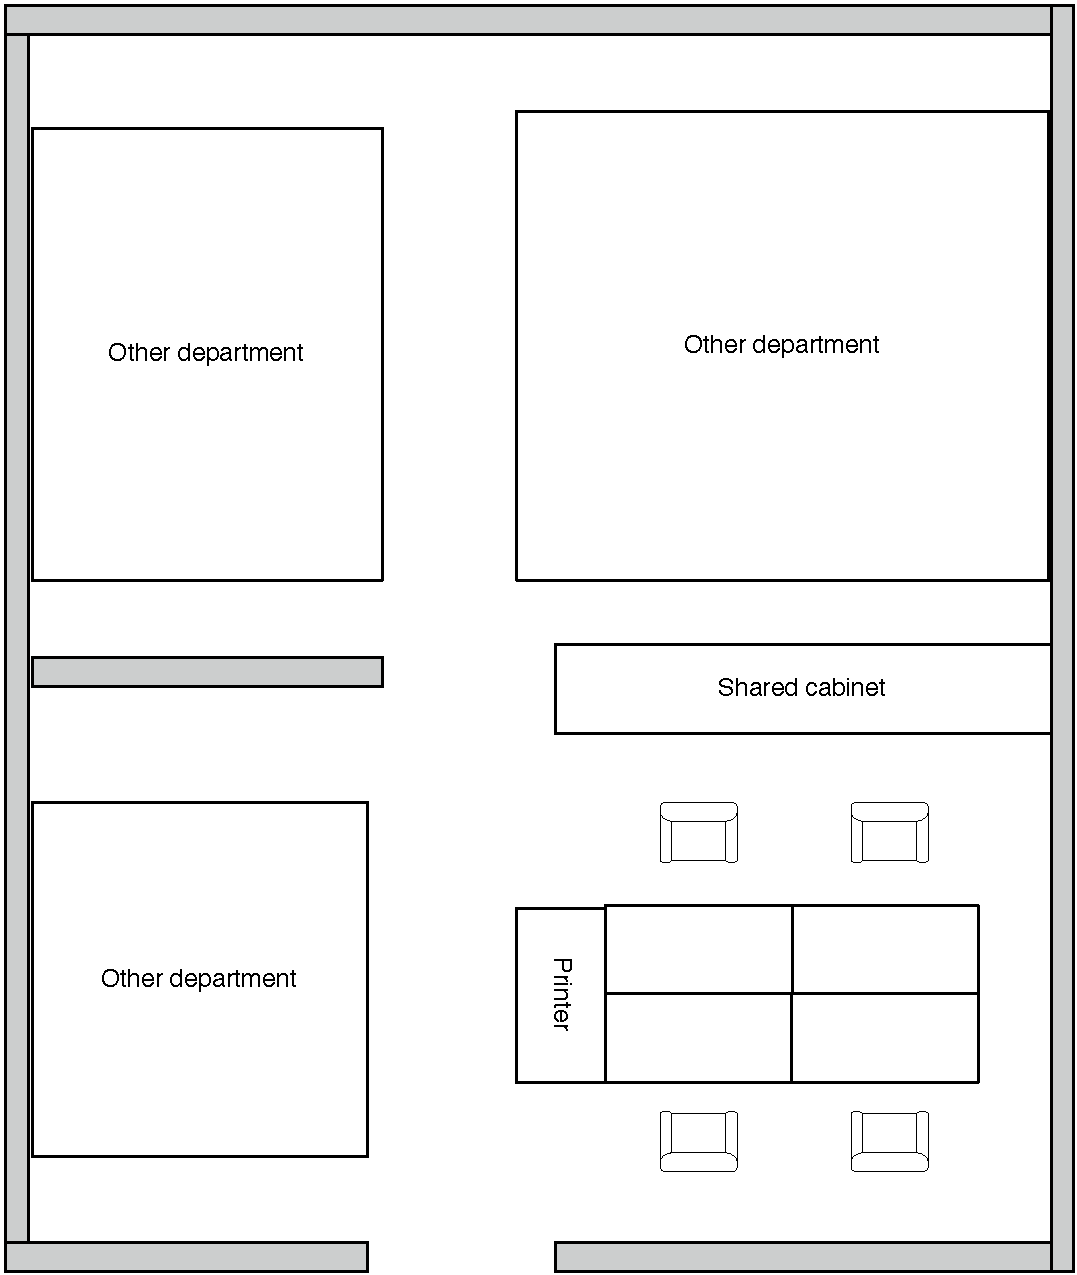
\includegraphics[width=0.3\textwidth]{images/ch12/ch12_physmodroom.pdf}
\caption[Study 2 Room model]{Physical model diagram showing a typical physical layout of people's work environment at room level.}
\vspace{-9pt}
\label{fig:ch12_physmodroom}
\end{figure}

\begin{figure}[!ht]
\centering
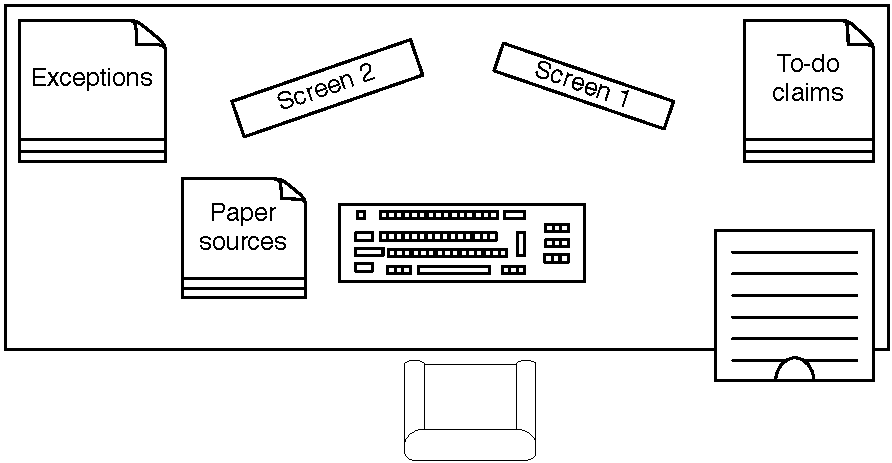
\includegraphics[width=0.3\textwidth]{images/ch12/ch12_physmoddesk.pdf}
\caption[Study 2 Desk model]{Physical model diagram showing the physical layout of people's work environment at desk level.}
\vspace{-9pt}
\label{fig:ch12_physmodroom}
\end{figure}

The physical model describes what the individual can physically hear, see, and access, and how information sources are laid out in the physical environment. In developing the model the following was considered: what is the proximity of, and access to, devices and people: what can be seen and heard from the individual's point of view?

\begin{framed}\noindent
\textbf{Physical model principles}

\begin{itemize}
\item Space and Cognition: how do people use the physical space to support their work
%\item Perceptual principle: what is the mapping between the spatial layout of information, and that which it represents
%\item Naturalness principle: does the form of how information is represented match the properties of what it represents
\item Subtle bodily supports: do people use their body to support their work
\item Situation awareness: are people informed of what is going on
\item Horizon of observation: what are people able to see and hear
\item Arrangement of equipment: how do people arrange their equipment
\end{itemize}

\end{framed}

%Physical layout
The physical layouts of the four offices were not identical, but shared a number of characteristics. All participants had their own desk and worked in an open office with two or more colleagues. P3 was the only person in the office responsible for data entry tasks. The other eight participants had colleagues in the same room who dealt with similar tasks. P1, P2, P8 and P9 also had colleagues in the same room that worked on different tasks. Colleagues that were working on different tasks were situated further away from them than other colleagues. As an example, the physical environment of the office of P1 and P2 is depicted in Figure \ref{fig:ch12_physmodroom} at room (a) and desk (b) level. The number of people in one room ranged from two to sixteen. 

The open layout made it easy for colleagues to interact with each other and share information between themselves. They could see when a colleague was present and available to consult. Participants regularly consulted colleagues in their room to retrieve information they could not find on any other sources. This information is given verbally, or a colleague directs the participant to the correct information source.

The offices had an open-door policy, meaning that workers could at any time be interrupted by people walking in. During the observations, participants were regularly interrupted by colleagues. They responded to it but used \textit{subtle bodily supports} to not lose track of where they were in the expenses task. For example, P3 responded verbally to a colleague but kept his kept his visual attention on the computer and tried to continue with the expenses task. When P1 was interrupted by a colleague, he placed a finger on the computer screen to remember where he was in the task.

%Sometimes it is colleagues at the same level of processing, sometimes it is people who are higher in the task hierarchy. For example, a boss who needs to check another colleague'��s entries can be collocated around a desk and query this colleague if something is incorrect. They can also view how many of the outstanding claims still need to be processed as they are on their colleague's desk.

%SOURCES
All participants worked with both paper and digital information sources. Several participants used the physical \textit{space} to organise their paper sources. P2 maintained separate physical locations on his desk for expense claims to be processed, expense claims that had been completed, and exceptional claims that required further attention. P7 also had paper sources fixed on his wall, which were visible from his desk. 

Other physical sources were located in an individual's drawer, in a shared bookcase or drawer in the same physical room. These were not visible from their desk, and participants had to physically move from their desk to retrieve and view this information. Participants could see whether a colleague is present or not, and whether they can consult them at that moment to request information. Recent physical files are kept in a closet in the same room, whereas older files and employee files are physically kept in another location. These older files were used less frequently.
If P6 received expense claims, she placed these in her drawer to return to later. If there were a lot of claims to be processed or if the participant started processing claims, these were placed on their desk. 

Participants become aware of new claim requests by batches of claim forms or receipts on their desk with a handwritten note, the claimant asking them in person, or when they check their e-mail and see a new e-mail by the claimant. For physical claims, they browse through them and place them either at a dedicated area on their desk or in their drawer, to return to later. P2, P3 and P6 re-ordered claims based on urgency. Claims that were more urgent were processed first. These could be claims by their boss, or claims with an explicit instruction that it was urgent. In addition, P2 sometimes grouped claims according to category. The reason for grouping them is that different categories of expenses can require other data fields to be filled in, and P2 felt it to be easier to do these particular type of claims together. Examples are travel expenses for which participants have to fill in the departure point and destination, or external lunches for which the name of the restaurant has to be filled in. Participants place exceptional claims in a separate physical location. For P2, this was in a separate tray in the top-left hand corner of his desk. By putting it in his \textit{horizon of observation}, he can see if there are still claims in this tray to be processed and return to at a later point in time. P2 starts each day by seeing if there are claims in this tray, and processes these first. P5 places exceptional claims in a separate drawer. They are not visible and she does not use any reminders, but returns to these when she sees fit.

Participants also received requests digitally through email. They could not place these in their horizon of observation. However, whether the claim requests were in physical or digital form, they always needed the physical receipts of expenses, before they could process a claim. Similar to physical claim forms, they had these receipts either in their drawer or on their desk, as a reminder that they still needed to process these claim requests.

Participants also created their own artefacts to aid them in their work. This includes physical artefacts, such as a spreadsheet with frequently used codes, as well as digital artefacts, such as a digital form to look up codes by person name. Participants could type in a name of a claimant, and the form populated codes related to one person. This made it easier for people to look up which account codes to charge the expenses to. 

Digital information sources included the data entry system, intranet, and external websites via their computer. Furthermore, they had digital files, such as PDF files, Excel spreadsheets, and Word documents stored on their desktop computer. The \textit{arrangement of equipment} was that seven out of nine participants had two screens. All seven participants mainly used one screen, both to enter and retrieve information. Some participants used a second screen to display their email inbox. If they received a notification of a new email, they would briefly glance to determine the urgency and importance of the email, but would try to continue with the expenses task. 

Sometimes a claim was checked by multiple people in the same room. Participants had \textit{situation awareness} of the progress of the claim as long as it was still in the same physical office. They could see the progress of expense claims by the pile on colleagues' desks, and could ask colleagues in person. Furthermore, they can overhear conversations on the phone and become aware of claims that require further attention. Participants can see their own screens and desks. They have to walk over or do additional physical actions in order to view what is on colleagues' desk.  

As soon as an expense claim was submitted to another office and physical location, the user would have little \textit{situation awareness} of the progress of the claim. The system did not have a visible status update, meaning participants can not see the progress of their claim once it has been submitted to Central Finance. As they do not receive updates, administrators and claimants often forget to keep paying attention to it and do not query it until they realise payment has not been processed yet. Often an error will have occurred and at this point the project may have finished and payment is no longer possible. If participants needed more information on the status of a claim, they needed to contact colleagues from another office via email and telephone, or they had to visit the other physical location.  Participants called colleagues from other departments with queries such as errors, and outstanding claims that had not been processed yet. They emailed claimants with queries such as if they do not agree with the expenses claimed, if they need further information, or if they have spotted an error.


%\begin{table}[htp]
%\centering
%\begin{tabular}{  l }
%\hline
%\textbf{ Physical} \\  
%Paper receipts \\  
%Personal files of employees \\  
%Written instructions by claimants \\  
%Paper claim forms \\
%Calculator \\
%Documents created by the participant
%\vspace{10pt} \\
%
%\textbf{Digital} \\ 
%E-mails \\ 
%The expenses entry system \\ 
%Excel spreadsheets \\ 
%Intranet \\ 
%External websites \\ 
%PDF files \\ 
%Calculator \\ 
%Documents created by the participant
%\vspace{10pt} \\
%
%\textbf{Other} \\ 
%Colleagues \\ \hline
%
%\hline
%\end{tabular}
%\caption[Study 2 information sources]{The information sources people needed for expenses tasks.}
%\label{table:ch12_infsources}
%\end{table}


\subsubsection{Artefact model}
The artefact model describes the artefacts that are used. 

\begin{framed}\noindent
\textbf{Artefact model principles}  \\
\begin{itemize}
\item Mediating artefacts: do people use any artefacts to support their work
\item Creating scaffolding: do people use the environment to simplify tasks, e.g. set reminders
\item Representation:goal parity: do people use artefacts to display the explicit relationship between the current and goal state of their work
\item Coordination of resources: how do people coordinate their information
\end{itemize}
\end{framed}

%. Participants have access to their intranet, where project information for the department such as project codes are stored. 

Participants work with both physical and digital artefacts. Table \ref{table:ch12_infsources} shows an overview of the information sources that were involved in an expenses task. For each instance of the task, several artefacts can be used, but there are two main artefacts that are used in each instance and are central to the expenses task: the paper receipts and the expenses entry system.
In addition to information sources, participants use several \textit{mediating artefacts} to support their work. Calculators are used to aid in calculating sums. Multiple tools were consulted to convert currencies: an external website, a tool on the intranet, and a tool included in the data-entry system itself. They use a physical tray on their desk to hold exceptional claims. They use a pen to annotate receipts and highlight which items on receipts to claim back.

Some of the participants \textit{created external scaffolding} to simplify their task. In particular, participants had difficulties remembering codes they needed to enter. P5 and P6 had made a personal spreadsheet with codes they used most frequently. P4 remembered old codes but had difficulties remembering new codes since they had changed 18 months ago. To look up codes, she used a spreadsheet created by the departmental manager where she could fill in old codes, that would populate the correct new code. 

\textit{The parity between the current and goal state} was displayed on the expenses system. Once a claim had been submitted, there would be a status update in the expenses system. This status reveals whether a claim is Pending, has been Paid, or whether Original receipts are required. As long as a claim was Pending however, there was however no insight into what is happening on the other side. Often a claim would be received but would be held because there was information missing. Participants would not know about this unless they explicitly contacted the office, and depending on the situation, they would often still not receive information on what was happening with a particular claim because the information was not centralised in Central Office and the person on the phone would not be able to look up what was happening with a particular claim.

In order to \textit{coordinate resources}, the intranet was intended as a central point for claimants, administrators and Central Finance officers to access the same information resources. Participants find the resources difficult to use, so people often end up making their own local copies and working with these instead. This supports them better in their work, but they can end up working with old and incorrect information if information gets updated. Examples of information sources used locally are claim forms: claimants keep working with local copies on their computer and do not download the new forms. They keep using old information such as old salaries and old project codes. Another example are spreadsheets with budget codes: administrators created and used their own spreadsheets with codes. If codes were updated, they were not aware and ended up working with old codes. 
There was an instruction manual to do expenses, to ensure everyone carried this routine task in the same way. Newcomers usually learnt how to do it from other people rather than this written manual, as the experience was that it was often easier and faster to learn it this way. This way of learning the activity again had the risk that some people were doing it in the old, incorrect way, and passed on this incorrect way of doing work to others.
In order to provide proof of expenses, people still had to provide hard-copy receipts. These need to be sent to Central Finance, but often get damaged and lost and the claimant and administrator will not know, but Central Finance will not know either so nothing will happen unless the administrator or claimant takes action and chases it. 

In order to prevent people from interrupting an expenses task, people were logged out of the data entry system after a period of inactive use and they had to restart the task from the beginning. This added cost to resume the task kept participants focused on the data entry task, and they were less likely to interrupt and switch to unrelated tasks. However, people often did not know beforehand what the cost to access information was going to be. Furthermore, it was also not clear after how long the timeout would occur [quote].

\subsubsection{Information flow model}
This model describes the flow of information through several actors for an expenses task.

\begin{framed}\noindent
\textbf{Information flow principles}
\begin{itemize}
\item Information movement: how does information move throughout the system
\item Information transformation: does the representation of information undergo changes
\item Information hubs: what are the main points where different information channels meet
\item Buffering: are there any buffers to uphold information
\item Communication bandwidth: how does communication take place
\item Informal communication: does informal communication take place in addition to formal communication
\item Behavioural trigger factors: are there any local factors that individuals respond to
\end{itemize}
\end{framed}

\begin{figure}[!ht]
\centering
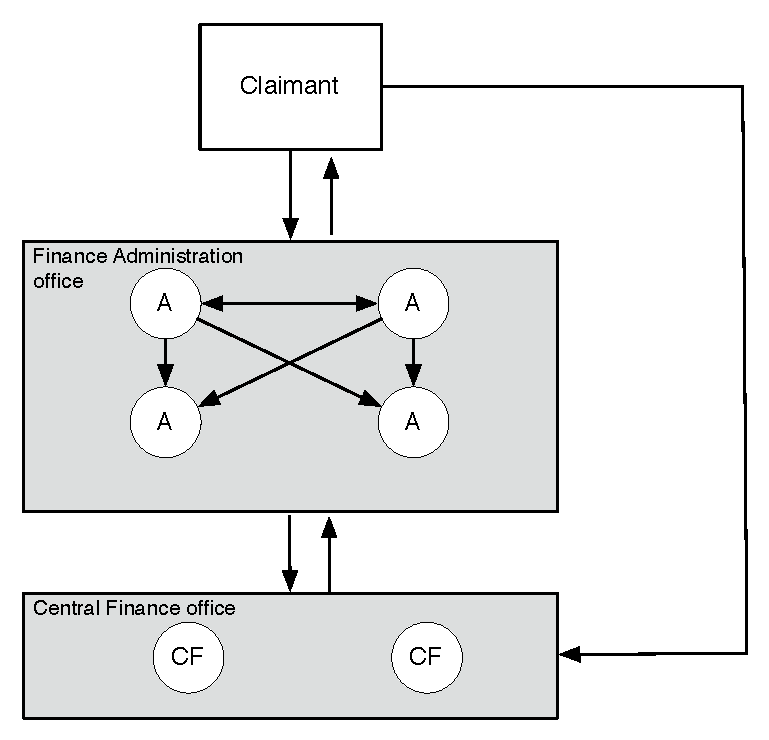
\includegraphics[width=0.3\textwidth]{images/ch12/ch12_infmodel.pdf}
\caption[Study 2 Information flow model]{Model of the information flow.}
\vspace{-9pt}
\label{fig:ch12_infmod}
\end{figure}


An expenses claim \textit{moves} through several actors, and moves between actors via email, phone, physical post, and face-to-face communication. The actors who contribute to the processing of an expense claim have limited visibility on the overall status and progress of the claim. For example, once claimants submit a claim request to the administrator, they do not know what the status is of that claim until they receive an email notification that it has been completed. Similarly, once administrators submit a claim to the Central Finance office, they do not know what the status is of the claim. They do not know when or whether it has been processed and if not, what the reasons are for holding it. The workers at the Central Finance office know the reasons for withholding a claim, but often receive incomplete information of a claim, and for example do not know the justification behind a claim, whether the expenses are made correctly and if there is an error in the project code entry, they do not know the correct project to charge it to.

\textit{Information transformation} takes place when calculations have to be carried out. At the beginning the individual numbers are saved, as well as the calculations on those numbers. Once a claim is submitted only the end result will be saved on the system. For example, if one claim request involves multiple expenses, each individual amount has to be checked by the administrator. Administrators are then free to choose whether to type each amount or only the sum total on the system. Once they have processed and submitted the claim, only the sum amount will be available for auditors. 

There are two main \textit{information hubs}: the first hub is the office of the administrator, who deals with incoming claims and hard-copy receipts from claimants. These claims are processed at the administrator office and then sent off to the Central Finance office, the second information hub. Workers at this office deal with incoming claims and hard-copy receipts from administrators, match and process these and submit them for payment. 

The administrator is the main\textit{ information buffer }between the claimant and the Central Finance officers. Claimants submit a request to administrators. This claim is upheld until the administrator decides to process it and send it to Central Finance. If there was an issue with a claim, claimants contacted the administrator, who then contacted Central Finance. Though claimants could also contact Central Finance directly, administrators said it was often easier if they contacted Central Finance on their behalf, as they knew who to contact [quote]. 

\textit{Communication} between the claimant and administrator takes place face-to-face, over the phone, via email and via handwritten notes. Communication between colleagues takes place face-to-face. Communication between the administrator and Central Finance solely takes part via email or over the phone, though it is possible to take place face-to-face.

Instructions are mostly \textit{communicated informally} through word of mouth. Knowledge of how to use the system sits with the employees, and it is often faster to explain newcomers how to do it rather than go through the written instructions. A consequence is that when information gets updated, not everyone is aware of it and keeps using the old and incorrect way, or learn the incorrect way from someone else who is still using the old way. 

Receiving a claim request from another actor are the main \textit{factors triggering behaviour.} Participants collected claim requests and saved them to return to later. Some participants kept claims to be completed on their desk. The size of this pile acted as a trigger to decide whether to start processing them. Furthermore, the payroll deadline was another trigger. Participants tried to complete claims before the deadline so claimants were reimbursed in time.

\subsubsection{Task strategies}
By describing the task environment, several strategies were uncovered. These are discussed in more detail below. After developing the models, the audio transcripts, notes, and video recordings were reviewed again to identify patterns of information strategies. 

\textbf{Planning for information needs}
Participants started processing an expense claim by collected all physical sources they knew they were going to need. These were the paper receipts, and could include a physical claim form and notes with written instructions. They placed this on a pile on their desk next to their computer, and entered this information first. 

Participants did not collect digital sources beforehand. Instead, participants retrieved these sources at the moment in the task they realised they needed it. When they realised they needed information from a digital source, they interrupted entering data, left the data entry window and went to search for the information. 

Participants did not always know beforehand what the cost of collecting this data was going to be, but assumed it could be retrieved fairly quickly. Sometimes it could take longer than expected due to various reasons. First, they did not always know which source to consult for finding the data. For example, people in Central Finance had to validate if the person signing off a claim form was authorised to give this signatory. The information to check this could be in a spreadsheet, but was sometimes also in a different PDF file. At other times, this information had to be looked up on the departmental intranet. Second, if participants did know which specific source to access, they did not always know the associated cost to access it. If information about a certain employee needed to be looked up, people consulted a search engine and typed in the person?s name. Sometimes they found the information quickly, but sometimes it took a while before they found what they needed. Third, even if participants did know the specific source and the normal cost, this cost was not always the same. For example, a website could take longer to load than usual.

If information was difficult to find, participants had time thresholds to decide whether to postpone it and come back to it later. P2 said that if he felt he was spending more than ten minutes on a task, he would postpone it. He placed uncompleted expense claims that required further attention in a separate tray on his desk. He revisited this pile the next morning and tried to process them then.
During observations, P5 could not find certain information for a claim either. After approximately five minutes of trying to find the information, she decided to write an email to the claimant requesting the information. She then put the claim form aside and started the next expenses task.
 
 \textbf{Creation of information sources}
Participants had access to shared files on the intranet of the office. They did not always find this information easy to use, and sometimes made their own local copies.
%Furthermore, collecting and organising information can be time-consuming (Bardram et al., 2006). This was also observed in the current study. 

\textbf{Deferral of interruptions}
In order to prevent people from interrupting an expenses task, people were logged out of the data entry system after a period of inactive use and they had to restart the task from the beginning. This added cost to resume the task kept participants focused on the data entry task, and they were less likely to interrupt and switch to unrelated tasks.
Participants did however interrupt a data entry task for task-related purposes, such as looking up information. They left the data entry interface and opened a new window. As windows were maximised, they were unable to see the data entry interface whilst they were looking up information. Participants explained it was much easier and faster to look up information on the screen they were already interacting with, rather than switch screens. They also felt that, opposed to physical sources, they could retrieve information from digital sources quickly. It sometimes took longer than expected however to look up certain information. Furthermore, it was also not clear how long the system would wait before logging them out. Upon coming back to the data entry interface, participants often found that they were logged out unexpectedly, needed to log back in and start from the beginning. In most cases, their information was lost.

\textbf{Use of multiple screens}
People dedicated one screen for the expenses task and maximised their window, so it filled the entire screen. This is in accordance with Bi and Balakrishnan (2009), who found that when dealing with two screens, people dedicate one computer screen to the primary task. However, they found that they use a second screen for subtasks. This was also found by Dearman and Pierce (2008)'s study on how people use multiple devices found that people assign sub-tasks to secondary devices to minimise the need to transfer information between devices.
People in the current study often also used their primary screen to look up information for the expenses task, and switched back and forth between maximised windows, rather than look up and display information on the second screen. In contrast, previous studies on the use of multiple screens showed that people dedicated a second screen to look up information \citep{Bi2009, Gurdin2001}. Even if people knew beforehand which digital information they were going to need, they often started the task and looked up information as they needed it. For paper information, they did collect all information they knew they were going to need, such as the paper receipts, the claim form, and any additional post-its with instructions. 
Whilst there was a possibility to place information on the second screen, this is also time-consuming \citep{Bardram2006}. With paper sources, it is perhaps less time-consuming: no time was spent on arranging the sources on the physical space of the desk, but they were stacked in a pile on their desk or lap and the right source was picked out when needed.
\citet{Dearman2008}'s study on how people use multiple devices found that people assign sub-tasks to secondary devices to minimise the need to transfer information between devices. Potentially people used the primary screen for looking up information so the information was on one screen and try could try to copy and paste it. Often though this was either not possible or users chose themselves to manually transcribe it.
 
People used additional screens for other tasks. For example, the second screen was often used to display the email inbox, but this was not consulted during the expenses task. Even in instances when people had to look up information from an email, they would open their inbox on the primary screen, rather than look it up on the second screen. 


\subsection{Discussion}
The purpose of this study was to investigate the information sources people need for an expenses task, and how they currently manage subtasks of looking up information from an expenses task.  Do they look up information as they need it, or get all the required information first and then enter it? Do they change their strategies as they get more experienced with the task and know where to get the information from?

The following questions were addressed:

\begin{enumerate}
\item 
What is the information needed for an expenses task?
\item 
Where is this information retrieved from?
\item 
What are the strategies people use to look up information?
\end{enumerate}

%WHAT INFORMATION AND WHERE FROM
\subsubsection{Information sources}
%Paper and digital sources
%Availability of information
The information needed for an expenses task needed to be retrieved from both paper sources, such as paper receipts, handwritten instructions and claim forms, as well as digital sources, such as spreadsheets, websites and emails.

The user did not always know beforehand what the cost of accessing digital sources was going to be. First, they did not always know which source to consult for finding the data. For example, people in Central Finance had to validate if the person signing off a claim form was authorised to give this signatory. The information to check this could be in a spreadsheet, but was sometimes also in a different PDF file. At other times, this information had to be looked up on the departmental intranet. Second, if participants did know which specific source to access, they did not always know the associated cost to access it. If information about a certain employee needed to be looked up, people consulted a search engine and typed in the person?s name. Sometimes they found the information quickly, but sometimes it took a while before they found what they needed. Third, even if participants did know the specific source and the normal cost, this cost was not always the same. For example, a website could take longer to load than usual.

Information was centrally available, but this was perceived as being difficult to use. As a result, users made their own local copies of information they needed and used these sources instead. Furthermore, procedural information was passed on via colleagues rather than the central information sources. This caused people to use outdated information. Multiple departments were involved in the task. There was no transparency of information and progress of activity, and explicit information exchange was needed. The system had a timeout to prevent long interruptions, but people still looked up information as they needed it. They often did not know the associated IAC and as a result were locked out. 

%WHAT ARE THE STRATEGIES PEOPLE USE
\subsubsection{Information strategies}
%Collect physical sources in a batch, before starting a task, %Lookup digital information as they need it 
With paper sources, no time was spent on arranging the sources on the physical space of the desk, but they were stacked in a pile on their desk or lap and the right source was picked out when needed.

People did not always know which information they were going to need for a task, which made it challenging to collect all information beforehand. Therefore, people usually started a task collecting physical sources they knew were needed, and looked up other information as they needed it. Even if people knew beforehand which digital sources they were going to need, they still looked up information as they needed it.

This is in contrast with \citet{Sohn2008}, who found that uncertainty of the location of information would cause people to leave looking for it until later. A difference with this study is that Sohn et al. (2008) looked at people?s information search behaviour for personal tasks. Perhaps there was a pressure for employees to finish their work tasks and the urgency of finishing the task weighed more than the potential time cost of looking up information.

%Use of multiple screens
People dedicated one screen for the expenses task and maximised their window, so it filled the entire screen. People in the current study often also used their primary screen to look up information for the expenses task, and switched back and forth between maximised windows, rather than look up and display information on the second screen. 

Previous studies on the use of multiple screens showed that people dedicated a second screen for subtasks that supported the main task, such as looking up information \citep{Bi2009, Dearman2008, Grudin2001}. Even if people knew beforehand which digital sources they were going to need, they often started the task without placing this on the second screen. They did not look up information until they needed it, and used their main screen for this.

Whilst there was a possibility to place information on the second screen, this is also time-consuming \citep{Bardram2006}. 
\citet{Dearman}'s study on how people use multiple devices found that people assign sub-tasks to secondary devices to minimise the need to transfer information between devices. Potentially people used the primary screen for looking up information so the information was on one screen and try could try to copy and paste it. Often though this was either not possible or users chose themselves to manually transcribe it.
 
People used additional screens for other tasks. For example, the second screen was often used to display the email inbox, but this was not consulted during the expenses task. Even in instances when people had to look up information from an email, they would open their inbox on the primary screen, rather than look it up on the second screen. This contrasts \citep{Grudin2001} where people deliberately used a second screen to look up information, even if it was  faster to retrieve it from their primary screen.

%Use of local copies

\subsubsection{Other issues}

\subsubsection{Contribution}
\begin{itemize}
\item
Evidence that an expenses task is fragmented: people often have to go in and out of the expenses system to look up information.    
\item
Evidence that the IAC of the required information sources for an expenses task varies. 
\item
Evidence that depending on people's experience and awareness of how costly it is to access information, they will try to minimise switching between tasks.
\end{itemize}

The goal of this study was to give an understanding of how people manage subtasks of looking up information as part of data entry work in a financial office.

\subsubsection{Limitations}
The goal of this study was to get an understanding of how people collect information as part of data entry work in a financial office. By using a Distributed Cognition approach, it became clear that information for an expenses task was not only distributed between external artefacts and internal cognition of one individual, but also between people. 
As the focus of analysis of this study was on the individual and not the team, the human agents are included as additional information sources. Studying distribution of cognition from a teamwork point of view is beyond the scope of this thesis, but will be useful to study in future work. Several issues became clear that related to teamwork, such as limitations in communication and coordination of central information. 

Due to confidentiality issues surrounding financial data, it was not possible to install logging software on participants' computers and all observational data reported here is qualitative. 
Given the situated nature of the study, it is also not clear to what extent people's behaviour is shaped by the access of the information sources, and how they are influenced by other situational factors such as user expertise. 
The next series of studies are set in a controlled environment, with the aim to study the influence of access costs to information on people's strategies, and how strategies impact quantitative performance measures as accuracy and speed. Study 1 and 2 have given an understanding of the task context and the information sources. The materials used in the subsequent studies will be designed to look similar to the office setting.
